\chapter{System Design}
\label{chap:system_design}

\section{High-Level System Architecture}
\label{sec:system_arch}
The Smart Driving Behaviour Analysis System is engineered as a decoupled, multi-tiered AIoT telematics platform. By isolating physical sensing from cloud analytics and visualization, the architecture guarantees fault tolerance, modularity, and real-time operational response. Figure~\ref{fig:system_arch} illustrates the high-level four-tier architecture.

\begin{figure}[H]
    \centering
    % Placeholder for System Architecture Diagram
    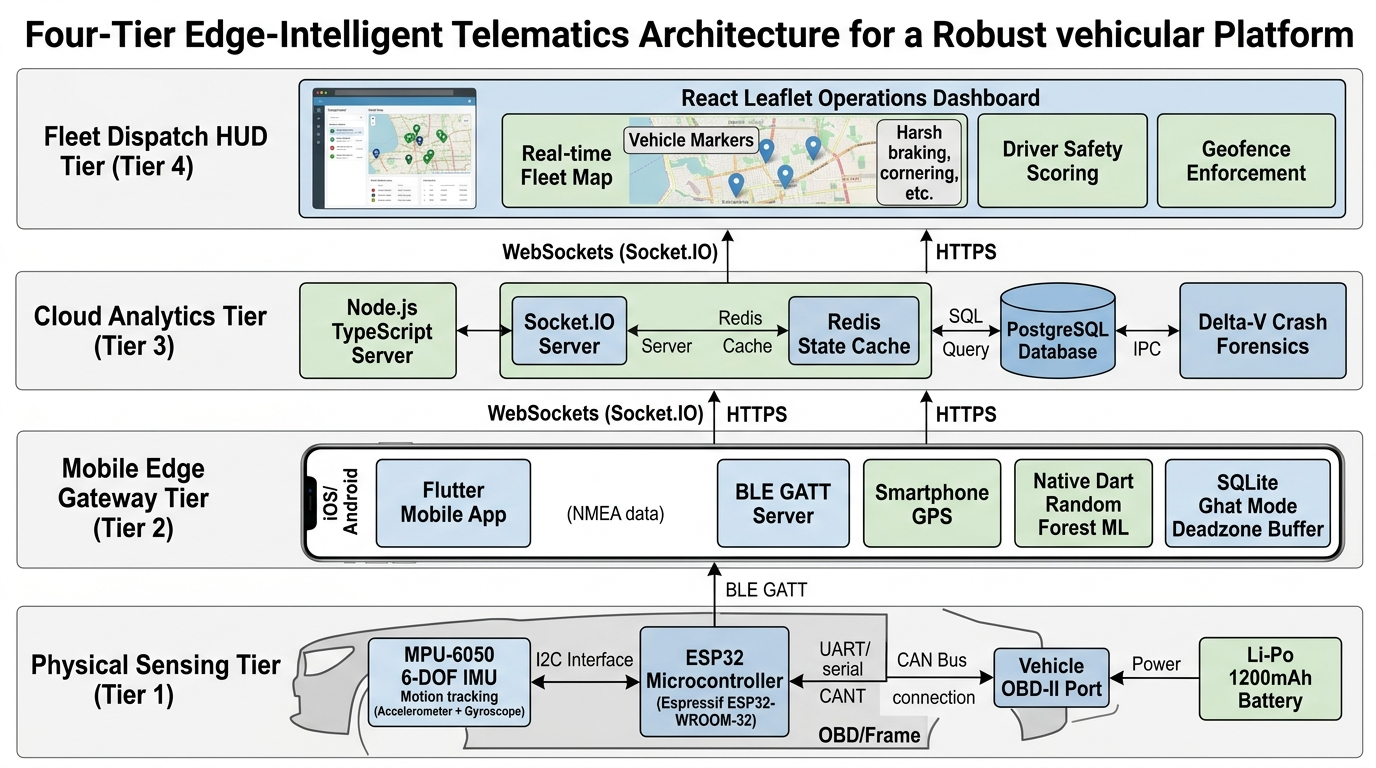
\includegraphics[width=0.88\textwidth]{figures/system_architecture.png}
    \caption{High-Level Four-Tier System Architecture of the Telematics Platform}
    \label{fig:system_arch}
\end{figure}

The four architectural tiers operate as follows:
\begin{enumerate}
    \item \textbf{Tier 1: Hardware Edge Sensing Node (ESP32 + MPU-6050):} 
    Rigidly fastened to the vehicle's structural frame, this node polls the 6-axis MEMS sensor via I2C at 20~Hz. It performs low-level register conversions, applies an onboard digital low-pass filter (DLPF), packs kinematic measurements into a 20-byte binary frame with a CRC16 checksum, and broadcasts the stream over a custom BLE GATT characteristic.
    
    \item \textbf{Tier 2: Mobile Gateway and Edge Preprocessor (Flutter Client):}
    The driver's mobile device acts as an intelligent edge gateway. It subscribes to the BLE telemetry characteristic, captures high-precision GPS spatial coordinates (1~Hz), and synchronizes the dual sensor streams. To conserve mobile resources and network payload, it applies a 3-meter spatial delta filter and maintains an offline FIFO ring buffer during cellular dead zones before transmitting HTTPS/WebSocket payloads to the cloud.
    
    \item \textbf{Tier 3: Cloud Microservices and Machine Learning Core (FastAPI \& PostgreSQL):}
    The cloud backend is powered by an asynchronous FastAPI microservice running under Uvicorn. Incoming telemetry batches are validated using Pydantic data schemas, processed through an Adaptive Exponential Moving Average (EMA) filter, and ingested by machine learning classification pipelines. The engine computes distance-normalized event rates, updates driver safety scores, and persists structured time series into PostgreSQL 15 and Redis 7.
    
    \item \textbf{Tier 4: Tactical Command and Control HUD (React 18 / Vite / Leaflet):}
    Fleet dispatchers and safety analysts interact with a web-based command center. The frontend displays real-time vehicle positions with dynamic heading orientation, renders color-coded trip breadcrumb routes, graphs instantaneous G-force telemetry, and alerts operators to high-G collision impulses or stationary anomalies.
\end{enumerate}

\section{Data Flow Modeling}
\label{sec:dfd}
The movement of information across system boundaries is modeled through structured Data Flow Diagrams (DFDs).

\subsection{DFD Level 0: Context Diagram}
The Level 0 Context Diagram establishes the macroscopic boundaries of the platform. The core system interacts with three primary external entities:
\begin{itemize}
    \item \textbf{Vehicle Edge Node / Driver:} Supplies raw 20~Hz kinematic telemetry vectors and GPS coordinates; receives real-time audio and visual driving coaching alerts.
    \item \textbf{Fleet Operations Manager:} Receives live fleet GIS maps, aggregated driver safety rankings, trip analytics, and incident reports; issues operational dispatch assignments.
    \item \textbf{Emergency Roadside Dispatch:} Receives automated SOS alerts containing vehicle coordinates, crash severity metrics ($\Delta V$), and driver contact details during critical impact anomalies.
\end{itemize}

\subsection{DFD Level 1: Subsystem Decomposition}
The Level 1 Data Flow Diagram decomposes the system into six distinct functional processes, as depicted in Figure~\ref{fig:dfd_level1}:
\begin{enumerate}
    \item \textbf{Process 1.0 (Telemetry Acquisition \& BLE Packing):} Captures raw ADC voltages from the MPU-6050, scales measurements to physical G-forces, validates CRC16 checksums, and transmits binary payloads over BLE.
    \item \textbf{Process 2.0 (Spatial Delta Filtering \& Gateway Fusion):} Fuses the BLE stream with smartphone GPS fixes and discards stationary breadcrumbs using a 3-meter displacement filter.
    \item \textbf{Process 3.0 (Digital Filtering \& Feature Extraction):} Applies an Adaptive EMA filter to suppress high-frequency chassis vibration, calculates first-order jerk derivatives, and extracts time-domain statistical features.
    \item \textbf{Process 4.0 (Maneuver Classification \& Anomaly Detection):} Evaluates feature vectors against supervised Random Forest models and deterministic threshold rules to identify harsh events and road potholes.
    \item \textbf{Process 5.0 (Driver Safety Scoring Engine):} Computes distance-normalized event rates ($\lambda_i$), applies non-linear exponential tolerance decay penalties, and derives the composite 0--100 safety score.
    \item \textbf{Process 6.0 (GIS Visualization \& Persistence):} Persists state data into PostgreSQL and Redis, broadcasting live updates to the React web dashboard via WebSockets.
\end{enumerate}

\begin{figure}[H]
    \centering
    % Placeholder for DFD Level 1 Diagram
    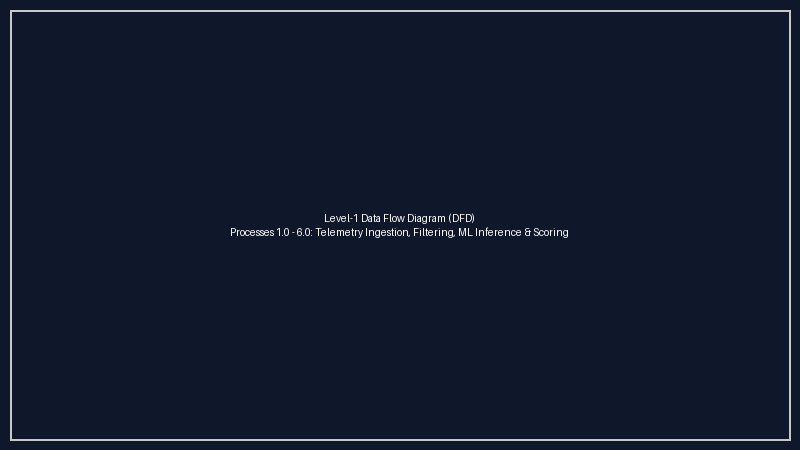
\includegraphics[width=0.85\textwidth]{figures/dfd_level1.png}
    \caption{Level 1 Data Flow Diagram (DFD) Illustrating Telemetry Ingestion and Analytics}
    \label{fig:dfd_level1}
\end{figure}

\section{Mathematical Formulations and Analytical Models}
\label{sec:math_models}

\subsection{Kinematic State Vector Representation}
At each discrete time index $k$ (sampled at $\Delta t = 50\text{ ms}$), the vehicle's instantaneous dynamic state is represented by a 14-dimensional kinematic telemetry vector:
\begin{equation}
    \vec{T}_k = \left[ \text{lat}_k, \, \text{lng}_k, \, v_k, \, \theta_k, \, a_{x,k}, \, a_{y,k}, \, a_{z,k}, \, \omega_{x,k}, \, \omega_{y,k}, \, \omega_{z,k}, \, \text{vib}_k, \, t_k, \, \text{driverId}, \, \text{tripId} \right]^T
\end{equation}
where $\text{lat}, \text{lng}$ represent WGS-84 coordinates, $v$ is ground speed in km/h, $\theta$ is vehicle azimuth heading ($0^\circ - 359^\circ$), $a_x, a_y, a_z$ denote tri-axial linear accelerations in G-force units ($1.0g \approx 9.80665\text{ m/s}^2$), $\omega_x, \omega_y, \omega_z$ denote angular rotational rates in rad/s, $\text{vib}$ is dynamic vibration amplitude, and $t$ is UTC Unix epoch timestamp.

\subsection{Adaptive Exponential Moving Average (EMA) Noise Filter}
To isolate genuine vehicle maneuvering dynamics from engine acoustic resonance and high-frequency road roughness, the raw acceleration signals pass through an Adaptive Exponential Moving Average (EMA) filter:
\begin{equation}
    y_t = \alpha_t \cdot x_t + (1 - \alpha_t) \cdot y_{t-1}
\end{equation}
The smoothing coefficient $\alpha_t$ dynamically adapts based on the magnitude of the vehicular jerk $|\dot{a}| = \left|\frac{x_t - x_{t-1}}{\Delta t}\right|$:
\begin{equation}
    \alpha_t = 
    \begin{cases}
        0.22, & \text{if } |\dot{a}| \le 1.5g/\text{s} \quad \text{(Cruising Mode: High Smoothing)} \\
        0.65, & \text{if } |\dot{a}| > 1.5g/\text{s} \quad \text{(Dynamic Event Mode: Rapid Tracking)}
    \end{cases}
\end{equation}
Additionally, a deadband threshold is enforced:
\begin{equation}
    y_t = 0, \quad \text{if } |y_t| < 0.06g
\end{equation}
This eliminates persistent zero-bias resting sensor drift during stationary vehicle idling.

\subsection{Spatial Displacement Filter}
Given two consecutive GPS positional fixes $P_1(\text{lat}_1, \text{lng}_1)$ and $P_2(\text{lat}_2, \text{lng}_2)$, the great-circle spatial displacement $d$ is determined via the Haversine formula:
\begin{equation}
    \Delta \phi = \frac{\pi}{180}(\text{lat}_2 - \text{lat}_1), \quad \Delta \lambda = \frac{\pi}{180}(\text{lng}_2 - \text{lng}_1)
\end{equation}
\begin{equation}
    a = \sin^2\left(\frac{\Delta \phi}{2}\right) + \cos\left(\frac{\pi \cdot \text{lat}_1}{180}\right)\cos\left(\frac{\pi \cdot \text{lat}_2}{180}\right)\sin^2\left(\frac{\Delta \lambda}{2}\right)
\end{equation}
\begin{equation}
    d = 2 R \cdot \text{atan2}\left(\sqrt{a}, \sqrt{1 - a}\right)
\end{equation}
where $R = 6371.0\text{ km}$ represents the mean radius of Earth. A telemetry coordinate update is persisted to the database if and only if $d \ge 3.0\text{ meters}$.

\subsection{Vertical-Dominant Road Surface Defect (Pothole) Model}
Potholes and road fissures induce localized vertical impacts without producing corresponding planar turning forces. A road defect anomaly is confirmed if:
\begin{equation}
    \begin{cases}
        v_k \ge 12.0\text{ km/h} \\
        |a_{z,k}| \ge 1.90g \\
        |a_{z,k}| > 1.25 \cdot \sqrt{a_{x,k}^2 + a_{y,k}^2} \quad \text{or} \quad |a_{z,k}| \ge 2.40g
    \end{cases}
\end{equation}
To prevent multiple detections for a single extended depression, a temporal debounce window of $\Delta t_{\text{debounce}} \ge 4.0\text{ seconds}$ is enforced between consecutive pothole alerts.

\subsection{Driver Safety Scoring Model}
The system implements an objective, distance-normalized mathematical scoring model. Let a trip span an effective distance $D_{\text{eff}} = \max(1.0, D_{\text{trip}})\text{ km}$. For each infraction category $i \in \{\text{braking}, \text{accel}, \text{speed}, \text{turn}, \text{phone}\}$, the distance-normalized event rate per 100~km is defined as:
\begin{equation}
    \lambda_i = \left(\frac{C_i}{D_{\text{eff}}}\right) \times 100
\end{equation}
where $C_i$ denotes the absolute count of detected infractions in category $i$.

Sub-penalties $P_i \in [0, 100]$ are calculated using an exponential tolerance decay function:
\begin{equation}
    P_i = 100 \cdot \left(1 - \exp\left(-\frac{\lambda_i}{\beta_i}\right)\right)
\end{equation}
where $\beta_i$ denotes the characteristic tolerance parameter for category $i$, parameterized as follows:
\begin{itemize}
    \item Harsh Braking: $\beta_{\text{brake}} = 6.0$
    \item Rapid Acceleration: $\beta_{\text{accel}} = 8.0$
    \item Overspeeding: $\beta_{\text{speed}} = 5.0$
    \item Sharp Turning / Swerving: $\beta_{\text{turn}} = 7.0$
    \item Distracted Phone Handling: $\beta_{\text{phone}} = 3.0$
\end{itemize}

The composite total penalty is computed as a convex linear combination of sub-penalties:
\begin{equation}
    P_{\text{total}} = w_{\text{brake}} P_{\text{brake}} + w_{\text{speed}} P_{\text{speed}} + w_{\text{turn}} P_{\text{turn}} + w_{\text{accel}} P_{\text{accel}} + w_{\text{phone}} P_{\text{phone}}
\end{equation}
with assigned weights $w = [0.25, 0.25, 0.20, 0.15, 0.15]$ such that $\sum w_i = 1.0$.

If a severe collision event is recorded ($C_{\text{crash}} > 0$), a safety floor condition is invoked:
\begin{equation}
    P_{\text{total}} = \max(P_{\text{total}}, \, 80.0)
\end{equation}

The final Driver Safety Score $S \in [0, 100]$ is given by:
\begin{equation}
    S = \max\left(0.0, \, \min\left(100.0, \, 100.0 - P_{\text{total}}\right)\right)
\end{equation}

\subsection{Collision Impulse Forensics ($\Delta V$)}
During a crash event, the structural impact impulse ($\Delta V$) is derived by integrating the high-G acceleration pulse across the crash duration $[t_0, t_1]$:
\begin{equation}
    \Delta V = \int_{t_0}^{t_1} \|\vec{a}(t)\| \, dt \approx \sum_{k=0}^{N} \|\vec{a}_k\| \cdot \Delta t
\end{equation}
where $\Delta V > 35\text{ km/h}$ designates a high-severity collision that automatically triggers the emergency SOS notification protocol.

\section{Database Schema Design}
\label{sec:db_schema}
The backend leverages PostgreSQL 15 structured relational storage optimized for time-series telemetry. Table~\ref{tab:db_schema} outlines the primary relational entities and their indexing schemes.

\begin{table}[H]
\centering
\small
\caption{PostgreSQL Relational Schema and Indexing Architecture}
\label{tab:db_schema}
\begin{tabularx}{\textwidth}{llp{5.5cm}l}
\toprule
\textbf{Table Name} & \textbf{Primary Key} & \textbf{Key Attributes} & \textbf{Indexing Strategy} \\
\midrule
\texttt{drivers} & \texttt{id} (UUID) & \texttt{name}, \texttt{license\_no}, \texttt{tier}, \texttt{reward\_pts} & B-Tree on \texttt{id} \\
\addlinespace
\texttt{trips} & \texttt{id} (UUID) & \texttt{driver\_id}, \texttt{start\_time}, \texttt{end\_time}, \texttt{distance\_km}, \texttt{avg\_speed}, \texttt{safety\_score} & Composite on \texttt{(driver\_id, start\_time)} \\
\addlinespace
\texttt{hazard\_events} & \texttt{id} (UUID) & \texttt{trip\_id}, \texttt{event\_type}, \texttt{latitude}, \texttt{longitude}, \texttt{severity}, \texttt{timestamp} & Spatial Index on \texttt{(lat, lng)}, B-Tree on \texttt{trip\_id} \\
\addlinespace
\texttt{telemetry\_logs} & \texttt{id} (BIGSERIAL) & \texttt{trip\_id}, \texttt{timestamp}, \texttt{speed}, \texttt{accel\_x}, \texttt{accel\_y}, \texttt{accel\_z}, \texttt{gyro\_z} & B-Tree on \texttt{(trip\_id, timestamp DESC)} \\
\bottomrule
\end{tabularx}
\end{table}
